\section{Introduction}

LLM serving increasingly manages persistent sessions rather than independent requests: a coding assistant, browser agent, or research copilot issues many model calls over minutes or hours, each depending on prior context, tool outputs, and intermediate state~\cite{yang2024sweagent,kwa2026measuring}. When a source cluster must shed load---maintenance, failure, traffic shifting, or a power-shed command---the system must decide where future requests run and how their serving state is rebuilt at the destination. Since prefill and decode stress different resources~\cite{zhong2024distserve,patel2024splitwise} and the KV cache is large and central to serving performance~\cite{kwon2023efficient,lmcache}, session movement becomes a resource-allocation problem over compute, bandwidth, cache state, and time.

\begin{figure}[t]
    \centering
    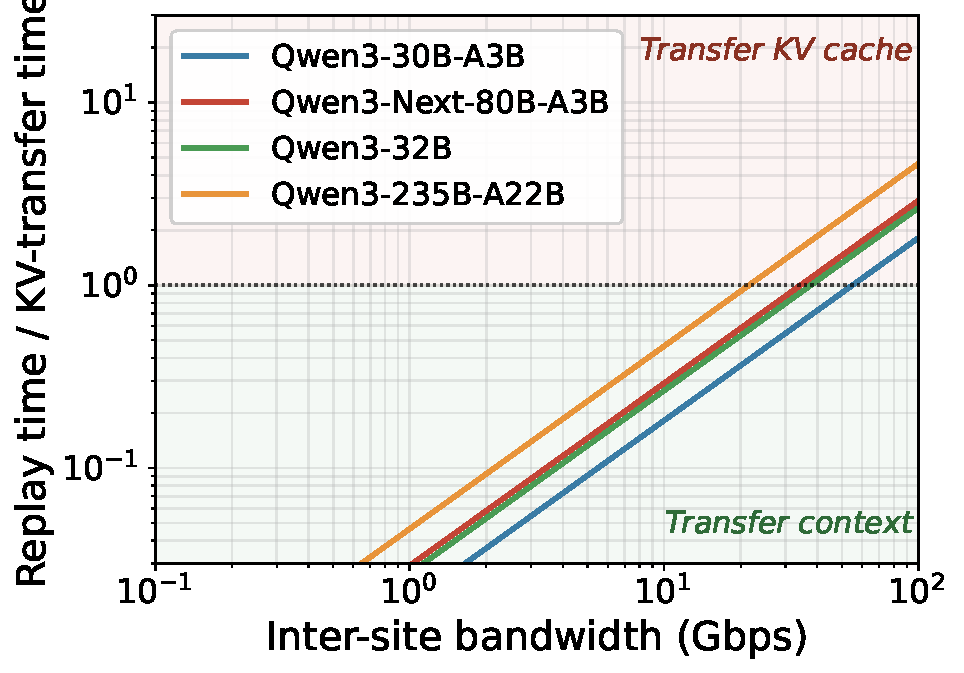
\includegraphics[width=\linewidth]{migration_ratio.pdf}
    \caption{
    Single-session replay/transfer boundary for a 100K-token context. The plot compares context replay against KV-cache transfer for several models. Values below the horizontal line indicate that transmitting context and recomputing KV through prefill is faster than transferring the KV cache. Values above the line indicate that KV transfer is faster.
    }
    \label{fig:migration-ratio}
\end{figure}

The simplest case is a single-session compute--communication tradeoff. A session can resume by transmitting its context and recomputing KV state through prefill, or by transmitting the KV cache and avoiding recomputation. Figure~\ref{fig:migration-ratio} plots this boundary for several models as inter-site bandwidth varies. Replay is preferable when bandwidth is limited or prefill is fast; KV transfer is preferable when bandwidth is high or prefill is expensive. For context length $T$, context size $\beta T$, KV size $\eta T$, prefill rate $\rho$, and bandwidth $\lambda$, replay is faster when
\[
    \underbrace{\frac{\beta T}{\lambda} + \frac{T}{\rho}}_{\text{context transfer and prefill}}
    <
    \underbrace{\frac{\eta T}{\lambda}}_{\text{KV transfer}},
\]
with crossover
\[
    \lambda^\star = \rho(\eta-\beta).
\]
This calculation identifies the basic parameters, but it only describes an isolated session.

A site-level shed couples many sessions through shared destination resources: replaying everything overloads prefill, while transferring all KV state congests the inter-site links. The policy problem is to allocate sessions across destinations and reconstruction actions while respecting bandwidth, prefill capacity, state-ingest capacity, and the required source-load reduction.

This project studies a convex relaxation of that allocation problem. We group sessions into classes by model and context length; for each class the decision is the fractional number of jobs sent to each destination under each reconstruction action, plus a \emph{stranded} count for jobs that miss the deadline. Replay is light on bandwidth but loads prefill; state transfer loads bandwidth and ingest but skips prefill. Both add reconstruction delay and deadline risk.

Rather than collapse the competing goals into one weighted cost, we solve a short \emph{lexicographic} stack of convex programs: migrate the most work under the deadline, then minimize peak resource pressure, then refine worst-class rebuild cost and cross-class fairness. The result is a continuous relaxation of the discrete placement problem---it does not model online scheduling or queueing, but it exposes the resource tradeoffs and gives a principled routing benchmark. We solve it exactly with CVXPY and study the Stage-2 dual: its congestion prices, an envelope-theorem sensitivity check, and subgradient / mirror-descent / ADMM attempts on the same dual. This report covers our progress---the exact solve recovers sensible replay/state structure and interpretable prices, while the first-order solvers are implemented but not yet tightly converged.